\section{Sampling Based Planners} \label{B. Sampling based planners}
A significant drawback of using resolution complete (the algorithm is guaranteed to find a path) and resolution optimal (the algorithm will find the shortest path if one is available) graph search planners such as A*, is that they are only suitable for small problem sizes \cite{gammell2014informed}.

The algorithms described in this chapter employ a sampling technique to explore the unknown environment rapidly, thus scaling well with large problem sizes.

\subsection{Rapidly-exploring Random Tree (RRT)} \label{sec: RRT}
The Rapidly-exploring Random Tree (RRT) \cite{lavalle1998rapidly, rodriguez2006obstacle, lavalle2001randomized, karaman2011sampling} is a randomised data structure solution to the pathfinding problem which shares some desirable properties with probabilistic road-maps (PRM) \cite{choset2005principles}, but, unlike PRMs, it is able to handle problems that have non-holonomic constraints (a holonomic robot is a robot which is able to move instantaneously in all available degrees of freedom).

The algorithm starts by creating a graph $G$ with a single vertex containing the agent position. Then, we proceed to incrementally add new vertices until we get to the goal region (the region in which we can assume that we have reached the goal or will be able to safely reach it). At each iteration, we sample a new point on the map which represents a valid position (not intersecting any obstacle, or out of bounds) $x_{rand} \notin Os$. We find the nearest vertex $x_{near}$ from $x_{rand}$ by searching the graph (e.g. graph pruning). We choose the next vertex to be inserted $x_{new}$ based on a predefined $max\_dist$ variable. If we are too far from $x_{near}$ ($d(x_{near}, x_{rand}) > max\_dist$) we choose a point on the line segment defined by $x_{near}$ and $x_{rand}$ that is $max\_dist$ far away from $x_{near}$. If we are too close to $x_{near}$ ($d(x_{near}, x_{rand}) \leq max\_dist$) we simply choose $x_{rand}$ (See Figure \ref{fig:RRT_new_node}). After we have chosen $x_{new}$, we make sure that the path from $x_{near}$ to $x_{new}$ is collision free, and if it is we add $x_{new}$ as a new vertex to the graph $G$ and $(x_{near}, x_{new})$ as a new edge (See Figure \ref{fig:RRT_example}, See Algorithm \ref{alg: RRT}).

It is worth mentioning that there exist some variations which use a dynamic $max\_dist$, usually picking a random number from the interval $[0, max)$ at each new iteration. Furthermore, the algorithm can be extended to different metric spaces by changing the distance function $d$.

\begin{figure}[]
  \centering
  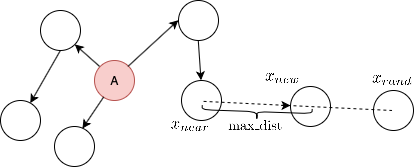
\includegraphics[scale=0.4]{images/RRT_new_node.png}
  \caption{RRT $x_{new}$ decision algorithm, if $x_{rand}$ is too far from $x_{near}$ we interpolate $x_{new}$ between the line segment defined by $x_{near}$ and $x_{rand}$ such that $x_{new}$ is $max\_dist$ away from $x_{near}$}
  \label{fig:RRT_new_node}
\end{figure}

\begin{figure}[]
  \centering
  \begin{subfigure}[b]{0.3\linewidth}
    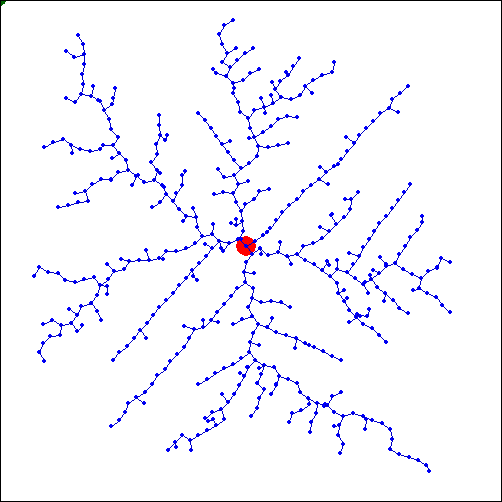
\includegraphics[width=\linewidth]{images/screenshot_40.png}
     \caption{500 iterations}
  \end{subfigure}
  \hfill
  \begin{subfigure}[b]{0.3\linewidth}
    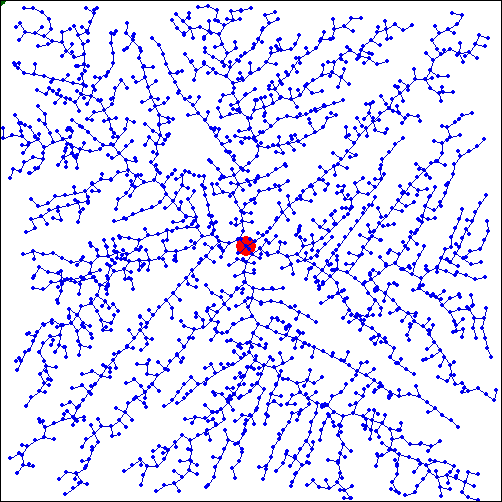
\includegraphics[width=\linewidth]{images/screenshot_41.png}
     \caption{2000 iterations}
  \end{subfigure}
  \hfill
  \begin{subfigure}[b]{0.3\linewidth}
    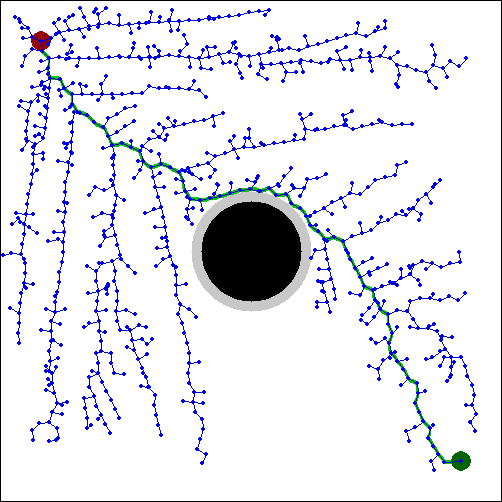
\includegraphics[width=\linewidth]{images/screenshot_39.png}
     \caption{Full RRT}
  \end{subfigure}
  \caption{RRT run with 500 iterations (left) and with 2000 iterations (middle) with $max\_dist$ 10. The whole algorithm can be seen in the right figure. Blue dots represent vertices and blue lines represent edges}
  \label{fig:RRT_example}
\end{figure}

\begin{algorithm}
\caption{Rapidly-exploring Random Tree (RRT)}
\label{alg: RRT}
\begin{algorithmic}[1]

\Procedure{RRT}{$M\colon(A, Os, G)$}
    \State $max\_dist \gets$ maximum distance
    allowed between tree children and sample
    \State $G \gets$ initalize graph with $A$ as vertex
    \While {True}
        \State $x_{rand} \gets \textit{Sample}()$
        \State $x_{near} \gets \textit{GetNearestVertex}(x_{rand})$
        \State $x_{new} \gets \textit{GetNewVertex}(x_{near}, x_{rand}, max\_dist)$
        \State
        \If {$\textit{CollisionFree}(x_{near}, x_{new})$}
            \State add $x_{new}$ as a new vertex to $G$
            \State add $(x_{near}, x_{new})$ as a new edge to $G$
        \EndIf
        \State
        \If {$x_{new}$ is in $G$ region}
            \State follow trace from root $G$ to $x_{new}$
            \State \Return 
        \EndIf
    \EndWhile
\EndProcedure
\end{algorithmic}
\end{algorithm}

Space complexity is $\mathcal{O}(|V| + |E|)$, where $|V|$ is the number of nodes and $|E|$ is the number of edges in graph $G$. Time complexity is given by $\mathcal{O}(i (\mathcal{O}(Sample) + \mathcal{O}(GetNearestVertex) + \mathcal{O}(GetNewVertex) + \mathcal{O}(CollisionFree)))$, where $i$ is the number of iterations and $\mathcal{O}(x)$ is the time complexity of method $x$. $i$ can be bounded by the number of nodes from graph $G$ ($\mathcal{O}(|V|)$) (at each step we add a new node to the graph). $\mathcal{O}(Sample)$ depends on the choice of sampling method (we use uniform random sampling which is $\mathcal{O}(1)$). $\mathcal{O}(GetNearestVertex)$ has DFS time and space complexity which is $\mathcal{O}(b^d)$ and $\mathcal{O}(bd)$, where $b$ is branching factor and $d$ is depth (if pruning is used $b$ becomes $\hat{b}$). $\mathcal{O}(GetNewVertex)$ is $\mathcal{O}(1)$ as it is a simple logical decision. $\mathcal{O}(CollisionFree)$ depends on the collision detection system. There are collision systems that have $\mathcal{O}(n)$ time complexity (for all entities). Because we need to check the path between $x_{near}$ and $x_{new}$ we still have $\mathcal{O}(n)$ time complexity. Therefore, the final time complexity is given by $\mathcal{O}(|V|(\mathcal{O}(b^d) + \mathcal{O}(n)))$.

A major advantage of using this method is that it is quite fast and memory efficient since it is run on a subset of the grid (the samples). Moreover, the algorithm can be coupled with the algorithms described in the Section \ref {C. Interpolating curve planners} (\hyperref[C. Interpolating curve planners]{Interpolating Curve Planners}) by transforming the graph edges into curves, which offers support for non-holonomic robots.

A major disadvantage is that, although the algorithm is probabilistic complete (as more samples are drawn the more likely is to find a path to the goal), it does not find an optimal path and the solution is usually quite jerky.

To overcome this issues, we introduce the RRT* \cite{karaman2011sampling, gammell2014informed} algorithm which has been proven to be asymptotic optimal (as the number of iterations gets larger, the more we approach to the optimal solution). RRT* does this by incrementally modifying the structure of the graph. When a new node is affixed to the graph, the algorithm might choose to rewire the connections in the graph by considering the new node as a replacement parent for the other existing nodes, if the resulting change yields a better solution. 

A major drawback of using RRT* is that, in order to achieve an optimal solution, the number of iterations has to be quite large and therefore, it becomes quickly expensive in higher dimensions. The Informed RRT* \cite{karaman2011sampling} algorithm attempts to solve this issue by adopting an ellipsoid heuristic approach. The algorithm shares the same logic as RRT* and it only improves the performance of finding an optimal path once a solution is found. This is achieved by sampling from the ellipsoidal heuristic. Thus, the number of iterations is reduced, and the optimal search is focused on a smaller region.

% \subsection{RRT*}

% Therefore, we introduce the RRT* \cite{karaman2011sampling} algorithm which is asymptotic optimal (as the problem size gets bigger, the more we approach to the optimal solution).

% % - prefers exploring the unexplored regions, large vornoi gaps
% % - good sampling from a smooth pdf Poisson Disc Sampling
% % - single nearest-neighbour queries

% \subsection{Informed RRT*}
% The informed RRT* \cite{gammell2014informed}
% %\subsection{Basic Probabilistic Road Map (Basic PRM)}